\documentclass[main.tex]{subfiles}

\begin{document}
\begin{figure}
    \center
    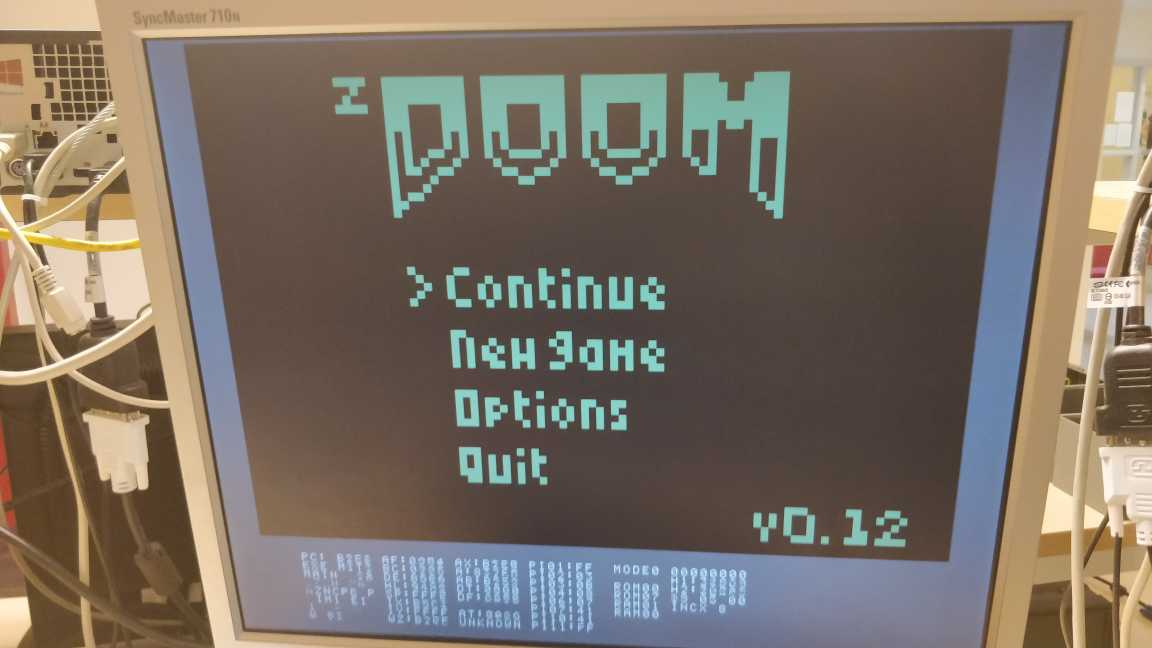
\includegraphics[width=0.8\textwidth,bb=0 0 1152 648]{img/monitor_small.jpg}
    \caption{Konstruktionens display vid körning av spelet zDoom.}
\end{figure}
\section{Konstruktion}
Det här avsnittet är en överblick av hur apparaten och de diverse komponenterna
hänger samman och hur styrningen av apparaten går till.
\subsection{Uppsättning}
\begin{figure}
    \center
    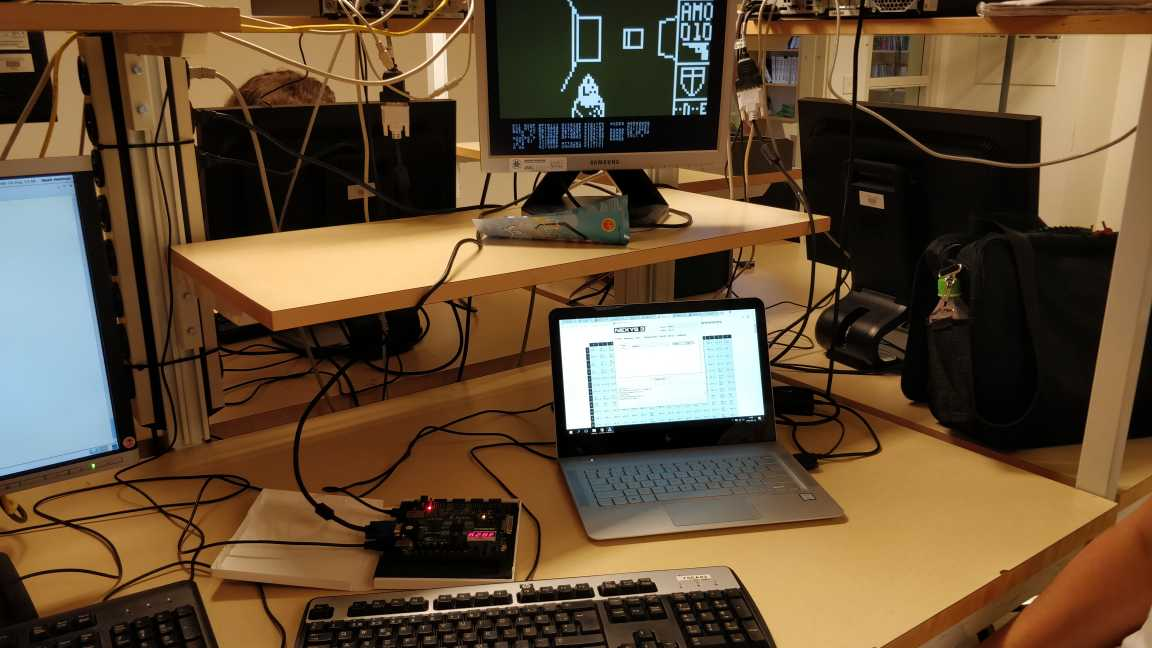
\includegraphics[width=0.8\textwidth,bb=0 0 1152 648]{img/setup_small.jpg}
    \caption{VGA-skärm och tangentbord kopplat till FPGA-kort tillsammans med
    laptop som används för att programmera FPGA:n samt ladda program till
    minnet.}
\end{figure}

FPGA kortet kopplas till en dator med programmet Adept [källa/länk] som används
för att hantera minnet hos FPGA-kortet. Programmet fanns inte på MUXens datorer
så en extern bärbar dator användes för att överföra datan. Tangenbordet är
kopplat till FPGA-kortets USB port för att kunna skicka indata till
FPGA-kortet. VGA-kabeln går till en 640x480 VGA-skärm.  Då miniräknaren har en
96x64 skärm har varje pixel skalats upp med faktorn 6.

\subsection{Användarhandledning}
% TODO beskriva hur man laddar allmänt program samt TI ROM
För att kunna köra ett av de program som laddas in måste de hamna på rätt
adresser i minnet. Adresserna väljs i Adept, en för TI83-romet och en för
användarens program. CPU:ns programräknare startar alltid på adress 8000 så ett
hopp laddas även in för att komma till användarminnet där programmet ligger.
Programmet som laddas in måste vara en binär fil för att FPGA:n ska kunna tolka
filen. Därför måste programmet först konverteras från assembly-kod till en
sådan fil. Konverteringen sker via z80asm som är en assembler för z80
instruktioner.

% TODO beskriva knappar, kommer inte ändras mer
Alla knappar, brytare, LED-lampor samt 7-segmentsdislayen på FPGA-kortet
användes i debuggingsyfte. Vad varje knapp gjorde ändrades ofta eftersom det
som skulle debuggas ständigt ändrades. Det är möjligt att stega T-cyklar,
instrukter samt ändra klockhastighet, sätta brytpunkter och lite annat som kan
vara lämpligt att ha i debuggingssyfte.

\clearpage
\end{document}
